
\documentclass[a4paper,12pt]{article}
\usepackage{epstopdf}
\usepackage[utf8]{inputenc}
\usepackage[swedish]{babel}
\usepackage{enumerate}
\usepackage{mathtools}
\usepackage{hyperref}
\usepackage{float}
\usepackage[pdftex]{graphicx}   
\usepackage{multirow}
\usepackage{listings}
\lstset{
    language=matlab,
    basicstyle=\ttfamily
}

\title{TBMI26  \\
       Assignment 1}
\author{Martin Estgren \texttt{<mares480>}}
      
\begin{document}
 \pagenumbering{arabic}
    \maketitle % Generate.
\section{Assignment 1}

\subsection{Overview of the data}

  
Looking at the data from a machine learning perspective we can observe how the data is compressed from 32x32 bitmap images to 64 features with the integer range 0..16. This means that we can create a hypercube feature space with 64 dimensions. This is a significantly dimensionally reduced feature space compared to 32x32 binary dimensions.

The pre-processing of the data doesn't only reduce the number of dimensions, it also reduces the variance in small distortions.

\subsection{Implementation of the kNN algorithm}

\subsubsection{kNN without cross-validation}
The implementation of kNN is fairly straight forward. 

We iterate though all the cases in the test set and calculate the distance to each point in the training set. The result is then sorted in ascending order and the `k` first elements are counted in regards to what label they are assigned. The label with the most values are then picked to be assigned for the testing case we are currently processing. When no counted label is higher than another we pick the label with the data point which have the closest euclidean distance to the test case.

The result of our implementation of the kNN algorithm with k arbitrarily choose as 4 can be seen below.

Parameters: k = 4
Accuracy = 0.9710

\begin{verbatim}
cM =

    99     0     0     0     0     0     0     0     0     0
     0    97     1     0     0     0     0     0     2     3
     0     0    97     0     0     0     0     0     0     1
     0     1     0    98     0     0     0     0     0     3
     0     1     0     0    96     0     0     0     0     2
     0     0     0     1     0   100     0     0     0     1
     1     0     0     0     0     0   100     0     0     0
     0     0     2     0     0     0     0   100     0     0
     0     1     0     0     1     0     0     0    96     2
     0     0     0     1     3     0     0     0     2    88
\end{verbatim}

\begin{figure}[H]
\centering
\caption{Result from kNN}\label{fig:kNN-result}
  \begin{minipage}[]{1\textwidth}
  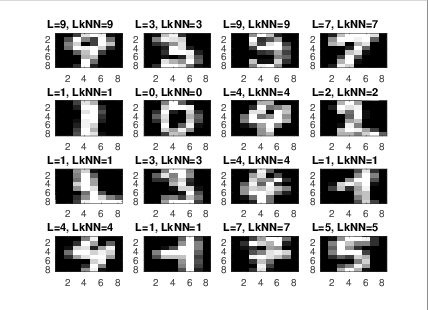
\includegraphics[width=\textwidth]{figures/kNN_simple.png}
  \end{minipage}
\end{figure}

\subsubsection{kNN with n-fold cross validation}

For the cross validation version the n-fold cross validation algorithm was used to determine the best value for k. For all of the following results $n = 2$ was used but he algorithm implementation allow for any value of n as long as it can evenly distribute the data set. Accuracy is used as the validation score in order to find the best value for k.


\noindent \textbf{Dataset 1}

\begin{figure}[H]
\centering
\caption{Cross validation score}\label{fig:kNN-1-cv-score}
  \begin{minipage}[]{1\textwidth}
  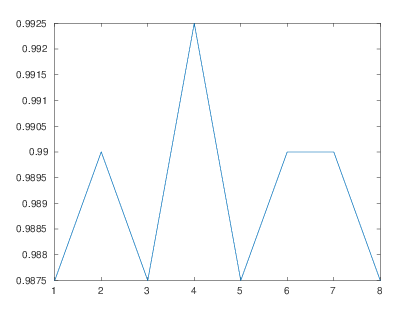
\includegraphics[width=\textwidth]{figures/kNN_1_cv_score.png}
  \end{minipage}
\end{figure}

\textbf{Best parameters:}
\begin{itemize}
\item $k = 1$
\item $Accuracy = 0.9900$
\end{itemize}

\begin{figure}[H]
\centering
\caption{Cross validation result}\label{fig:kNN-1-cv}
  \begin{minipage}[]{1\textwidth}
  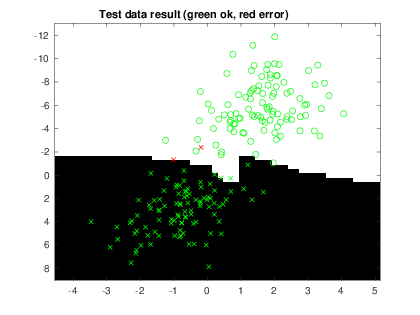
\includegraphics[width=\textwidth]{figures/kNN_1_cv.png}
  \end{minipage}
\end{figure}

\noindent \textbf{Dataset 2}

\begin{figure}[H]
\centering
\caption{Cross validation score}\label{fig:kNN-2-cv-score}
  \begin{minipage}[]{1\textwidth}
  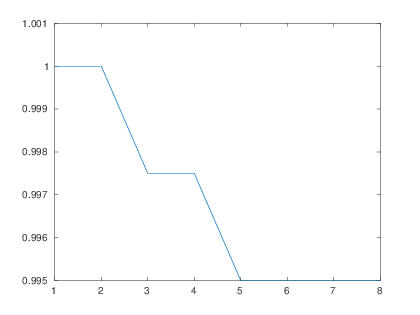
\includegraphics[width=\textwidth]{figures/kNN_2_cv_score.png}
  \end{minipage}
\end{figure}

\textbf{Best parameters:}
\begin{itemize}
\item $k = 1$
\item $Accuracy = 1$
\end{itemize}

\begin{figure}[H]
\centering
\caption{Cross validation result}\label{fig:kNN-2-cv}
  \begin{minipage}[]{1\textwidth}
  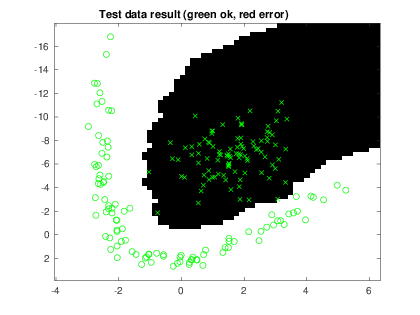
\includegraphics[width=\textwidth]{figures/kNN_2_cv.png}
  \end{minipage}
\end{figure}


\noindent \textbf{Dataset 3}

\begin{figure}[H]
\centering
\caption{Cross validation score}\label{fig:kNN-3-cv-score}
  \begin{minipage}[]{1\textwidth}
  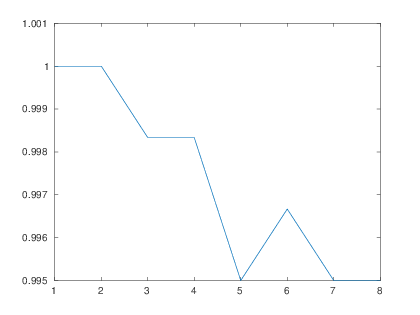
\includegraphics[width=\textwidth]{figures/kNN_3_cv_score.png}
  \end{minipage}
\end{figure}

\textbf{Best parameters:}
\begin{itemize}
\item $k = 1$
\item $Accuracy = 1$
\end{itemize}

\begin{figure}[H]
\centering
\caption{Cross validation result}\label{fig:kNN-3-cv}
  \begin{minipage}[]{1\textwidth}
  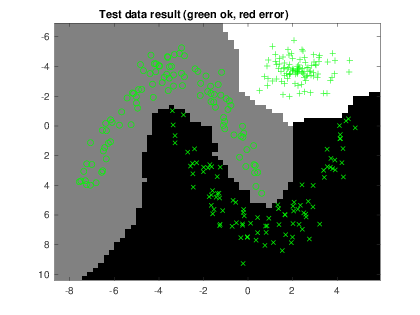
\includegraphics[width=\textwidth]{figures/kNN_3_cv.png}
  \end{minipage}
\end{figure}


\noindent \textbf{Dataset 4}

\begin{figure}[H]
\centering
\caption{Cross validation score}\label{fig:kNN-4-cv-score}
  \begin{minipage}[]{1\textwidth}
  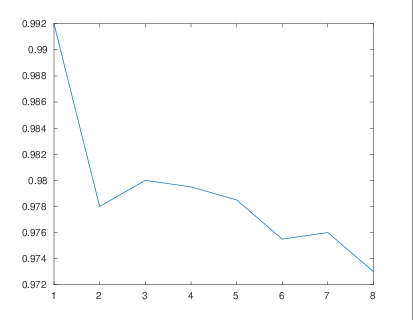
\includegraphics[width=\textwidth]{figures/kNN_4_score.png}
  \end{minipage}
\end{figure}

\textbf{Best parameters:}
\begin{itemize}
\item $k = 1$
\item $Accuracy = 0.9840$
\end{itemize}

\begin{figure}[H]
\centering
\caption{Cross validation result}\label{fig:kNN-4-cv}
  \begin{minipage}[]{1\textwidth}
  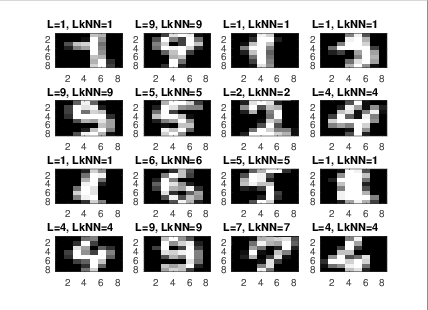
\includegraphics[width=\textwidth]{figures/kNN_4_cv.png}
  \end{minipage}
\end{figure}

\subsection{Single/Multi-layer neural network}

\subsubsection{Single layer backpropagation}

The implementation of the single layer backpropagation algorithm we use a linear activation function and the gradient $\frac{n}{s}(Y-Dt)*Xt^t$ where $n$ is the number of case, $Y$ is the result from the forward propagation, $Dt$ is the expected value for $Y$ and $Xt$ is a matrix with all training features.


\noindent \textbf{Dataset 1}

This is not a large feature space meaning we don't need huge precision in our weights.

\textbf{Parameters:}
\begin{itemize}
\item $Iterations = 800$
\item $learning rate = 0.005$
\item $Accuracy = 0.9950$
\end{itemize}
\begin{figure}[H]
\centering
  \begin{minipage}[]{0.49\textwidth}
  \caption{Single-layer network error}\label{fig:single_1_error}
  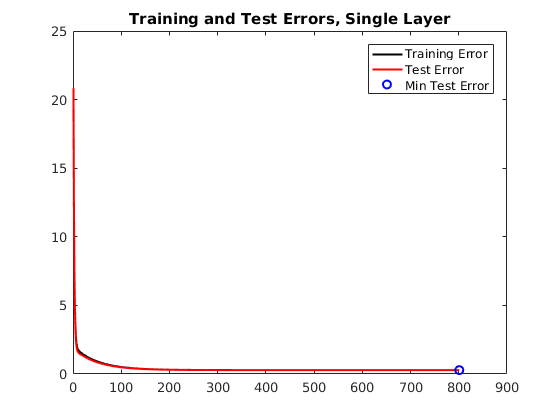
\includegraphics[width=\textwidth]{figures/single_1_error.png}
  \end{minipage}
  \begin{minipage}[]{0.49\textwidth}
  \caption{Single-layer network result}\label{fig:single_1_test}
  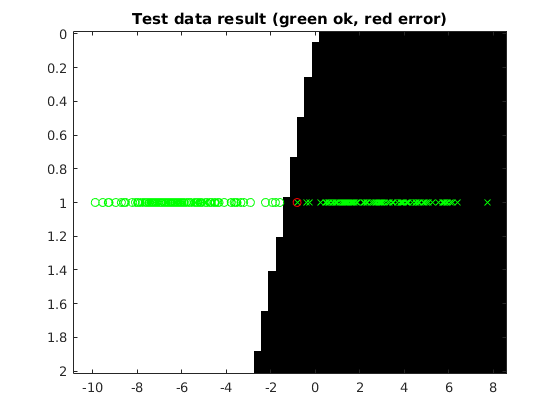
\includegraphics[width=\textwidth]{figures/single_1_test.png}
  \end{minipage}
\end{figure}

\noindent \textbf{Dataset 2}

For this data set we require much more precision which is why we have bumped up the number of iterations and reduced the learning rate.

\textbf{Parameters:}
\begin{itemize}
\item $Iterations = 200000$
\item $learning rate = 0.00005$
\item $Accuracy = 0.8200$
\end{itemize}

\begin{figure}[H]
\centering
  \begin{minipage}[]{0.49\textwidth}
  \caption{Single-layer network error}\label{fig:single_2_error}
  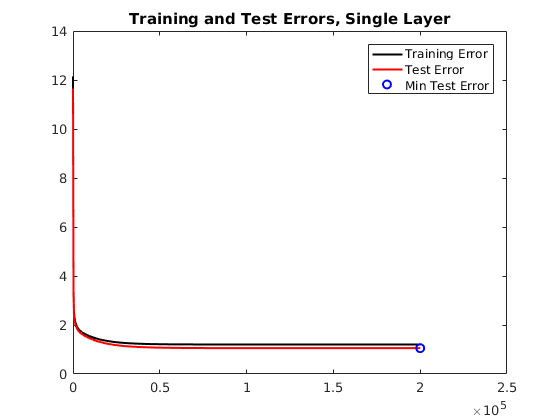
\includegraphics[width=\textwidth]{figures/single_2_error.png}
  \end{minipage}
  \begin{minipage}[]{0.49\textwidth}
  \caption{Single-layer network result}\label{fig:single_2_test}
  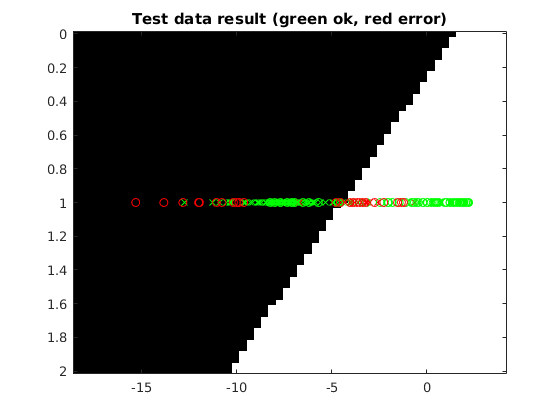
\includegraphics[width=\textwidth]{figures/single_2_test.png}
  \end{minipage}
\end{figure}

\noindent \textbf{Dataset 3}

These parameters should work just fine for this data set as well since we are classifying something that is similar to the last data set.

\textbf{Parameters:}
\begin{itemize}
\item $Iterations = 200000$
\item $learning rate = 0.00005$
\item $Accuracy = 0.8533$
\end{itemize}

\begin{figure}[H]
\centering
  \begin{minipage}[]{0.49\textwidth}
  \caption{Single-layer network error}\label{fig:single_3_error}
  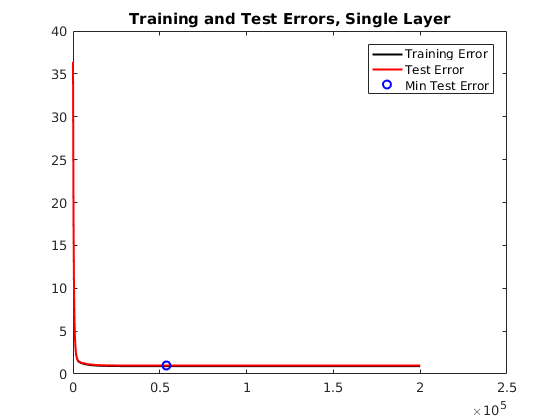
\includegraphics[width=\textwidth]{figures/single_3_error.png}
  \end{minipage}
  \begin{minipage}[]{0.49\textwidth}
  \caption{Single-layer network result}\label{fig:single_3_test}
  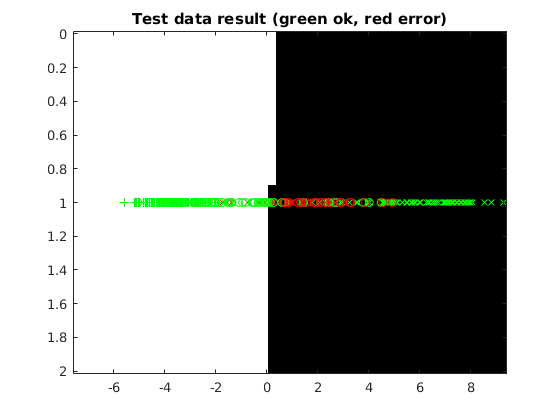
\includegraphics[width=\textwidth]{figures/single_3_test.png}
  \end{minipage}
\end{figure}

\noindent \textbf{Dataset 4}

This data set is much more complex compared to the other three but we are still dealing with the same number of neurons.

\textbf{Parameters:}
\begin{itemize}
\item $Iterations = 200000$
\item $learning rate = 0.00005$
\item $Accuracy = 0.9160$
\end{itemize}

\begin{figure}[H]
\centering
  \begin{minipage}[]{1\textwidth}
  \caption{Single-layer network error}\label{fig:single_4_error}
  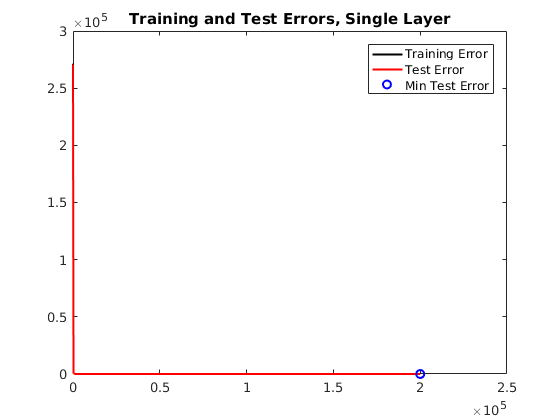
\includegraphics[width=\textwidth]{figures/single_4_error.png}
  \end{minipage}
\end{figure}

\begin{figure}[H]
\centering
  \begin{minipage}[]{1\textwidth}
  \caption{Single-layer network result}\label{fig:single_4_test}
  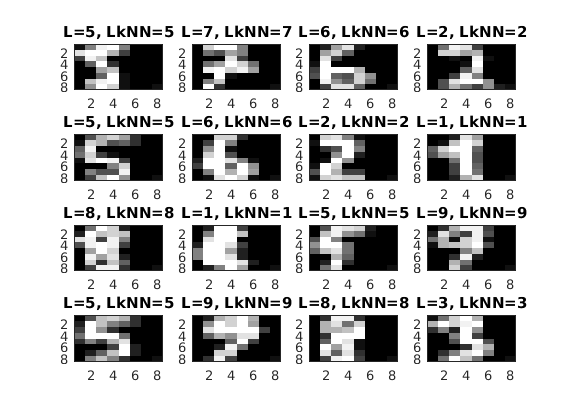
\includegraphics[width=\textwidth]{figures/single_4_test.png}
  \end{minipage}
\end{figure}


\subsubsection{Multi-layer backpropagation}

When dealing with multi layer networks we have to take care of order-of-magnitudes more number of weights. Because of this we want to limit the number of hidden neurons as much as we can. We are also using a non-linear activation function for the hidden layer which means we get transformed information at the linear output layer.

\noindent \textbf{Dataset 1}

For this dataset we progressively increased the number of hidden neurons, iterations, and lowered the learning rate until we got within out goal $Accuracy$

\textbf{Parameters:}
\begin{itemize}
\item $Hidden = 5$
\item $Iterations = 2000$
\item $learning rate = 0.01$
\item $Accuracy = 0.9950$
\end{itemize}

\begin{figure}[H]
\centering
  \begin{minipage}[]{0.49\textwidth}
  \caption{Multi-layer network error}\label{fig:multi_1_error}
  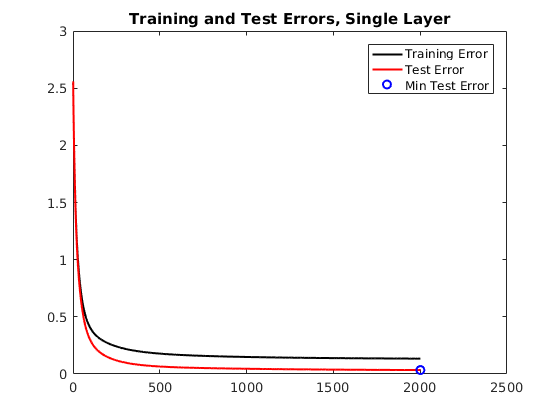
\includegraphics[width=\textwidth]{figures/multi_1_error.png}
  \end{minipage}
  \begin{minipage}[]{0.49\textwidth}
  \caption{Multi-layer network result}\label{fig:multi_1_test}
  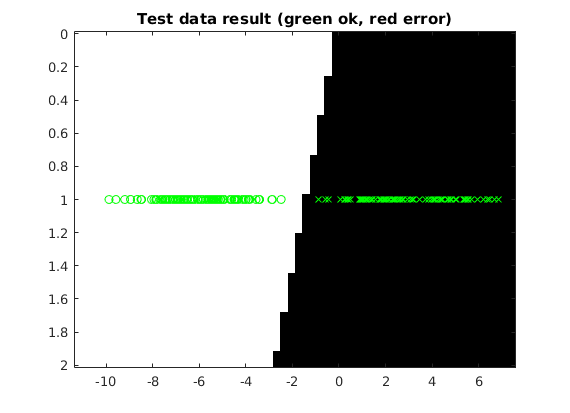
\includegraphics[width=\textwidth]{figures/multi_1_test.png}
  \end{minipage}
\end{figure}

\noindent \textbf{Dataset 2}

For this dataset we progressively increased the number of hidden neurons, iterations, and lowered the learning rate until we got within out goal $Accuracy$

\textbf{Parameters:}
\begin{itemize}
\item $Hidden = 2$
\item $Iterations = 30000$
\item $learning rate = 0.005$
\item $Accuracy = 1$
\end{itemize}

\begin{figure}[H]
\centering
  \begin{minipage}[]{0.49\textwidth}
  \caption{Multi-layer network error}\label{fig:singlemulti_2_error}
  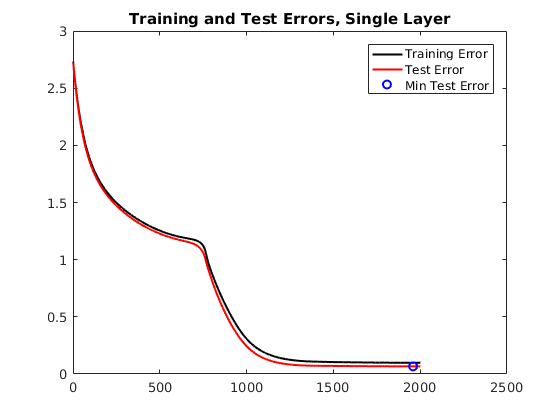
\includegraphics[width=\textwidth]{figures/multi_2_error.png}
  \end{minipage}
  \begin{minipage}[]{0.49\textwidth}
  \caption{Multi-layer network result}\label{fig:multi_2_test}
  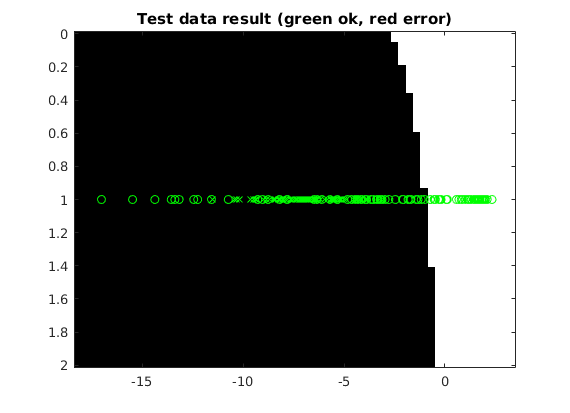
\includegraphics[width=\textwidth]{figures/multi_2_test.png}
  \end{minipage}
\end{figure}

\noindent \textbf{Dataset 3}

For this dataset we progressively increased the number of hidden neurons, iterations, and lowered the learning rate until we got within out goal $Accuracy$

\textbf{Parameters:}
\begin{itemize}
\item $Hidden = 10$
\item $Iterations = 4000$
\item $learning rate = 0.005$
\item $Accuracy = 0.9967$
\end{itemize}

\begin{figure}[H]
\centering
  \begin{minipage}[]{0.49\textwidth}
  \caption{Multi-layer network error}\label{fig:multi_3_error}
  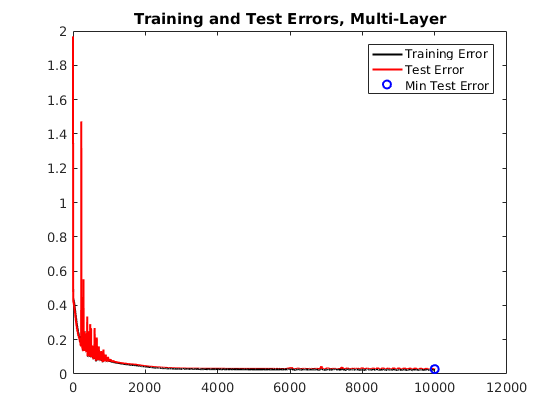
\includegraphics[width=\textwidth]{figures/multi_3_error.png}
  \end{minipage}
  \begin{minipage}[]{0.49\textwidth}
  \caption{Multi-layer network result}\label{fig:multi_3_test}
  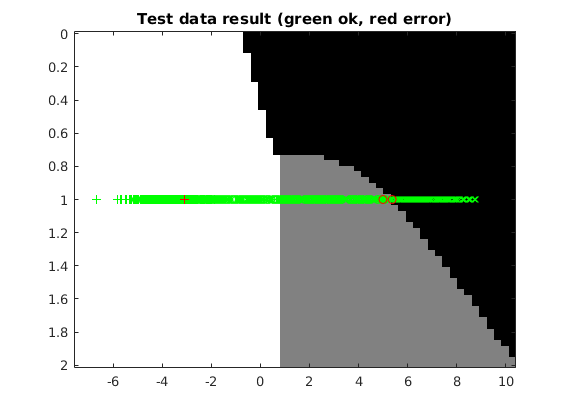
\includegraphics[width=\textwidth]{figures/multi_3_test.png}
  \end{minipage}
\end{figure}

\noindent \textbf{Dataset 4}

This dataset is a bit different, we are not dealing with only two or three dimension but 64. Because of the added complexity we can't find good parameters trough arbitrary guessing. Instead we set the number of hidden  to ten times the dimension, ensuring we get a model complex enough to find most approximate polynomials in 64 dimensions.

\textbf{Parameters:}
\begin{itemize}
\item $Hidden = 640$
\item $Iterations = 400000$
\item $learning rate = 0.001$
\item $Accuracy = 0.9150$
\end{itemize}

\begin{figure}[H]
\centering
  \begin{minipage}[]{1\textwidth}
  \caption{Multi-layer network error}\label{fig:multi_4_error}
  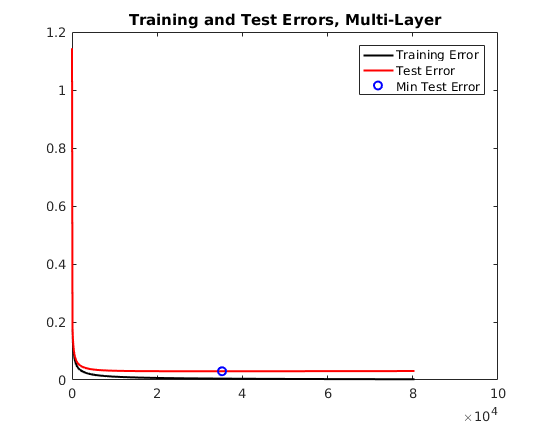
\includegraphics[width=\textwidth]{figures/multi_4_error.png}
  \end{minipage}
\end{figure}

\begin{figure}[H]
\centering
  \begin{minipage}[]{1\textwidth}
  \caption{Multi-layer network result}\label{fig:multi_4_test}
  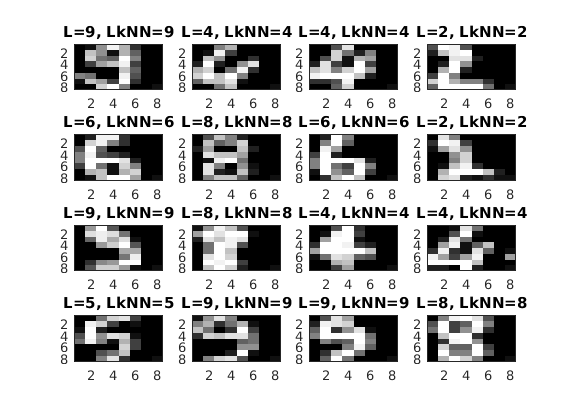
\includegraphics[width=\textwidth]{figures/multi_4_test.png}
  \end{minipage}
\end{figure}

\subsubsectino{Non-generalizable dataset}

If there's enough data points in order to find a reliable model for a unknown function we say that the model we get is non-generalizable. 


\end{document}
